%% ============================================================
%% MKT4846 -- Step 7 Writeup
%% Yildiz Technical University
%% ============================================================
\documentclass[12pt, a4paper]{article}

\usepackage[a4paper, top=2.5cm, bottom=2.5cm, left=2.5cm, right=2.5cm]{geometry}
\usepackage[utf8]{inputenc}
\usepackage[T1]{fontenc}
\usepackage{lmodern}
\usepackage{microtype}
\usepackage{graphicx}
\usepackage{booktabs}
\usepackage{array}
\usepackage{amsmath}
\usepackage{parskip}
\usepackage{fancyhdr}
\usepackage{titlesec}
\usepackage{xcolor}
\usepackage{hyperref}
\usepackage{caption}
\usepackage{subcaption}
\usepackage{float}
\usepackage{enumitem}

\definecolor{navyblue}{RGB}{15,32,60}
\definecolor{accentblue}{RGB}{30,90,170}
\definecolor{lightgray}{RGB}{245,245,248}

\hypersetup{colorlinks=true, linkcolor=accentblue, urlcolor=accentblue}

%% Section style
\titleformat{\section}{\large\bfseries\color{navyblue}}{}{0em}{}
\titlespacing*{\section}{0pt}{18pt}{8pt}

%% Header / Footer -- only active after cover page
\fancyhf{}
\fancyhead[L]{\small\color{gray} MKT4846 --- Camera-Lidar Sensor Fusion}
\fancyfoot[C]{\small\color{gray}\thepage}
\renewcommand{\headrulewidth}{0.3pt}

\captionsetup{font=small, labelfont=bf}

%% ============================================================
\begin{document}
\setlength{\parindent}{0pt}
\setlength{\parskip}{8pt}

%% -- COVER PAGE ---------------------------------------------
\thispagestyle{empty}

\begin{center}
\vspace*{1.5cm}

%% Logo
\includegraphics[height=5.6cm]{ytu_logo.png}

\vspace{1.2cm}
{\Large\bfseries Y\i{}ld\i{}z Technical University}\\[6pt]
{\normalsize Faculty of Mechanical Engineering, Department of Mechatronics Engineering}\\[4pt]
{\normalsize MKT4846 - Introduction to Autonomous Mobile Vehicles}

\vspace{1.8cm}
\noindent\rule{\textwidth}{1.2pt}\\[10pt]
{\LARGE\bfseries\color{navyblue} Camera-Lidar Sensor Fusion}\\[8pt]
{\large on the Waymo Open Dataset}\\[10pt]
\noindent\rule{\textwidth}{1.2pt}

\vspace{2cm}

\renewcommand{\arraystretch}{1.5}
\begin{tabular}{r@{\hspace{0.8em}:\hspace{0.8em}}l}
  \textbf{Name}       & Fatih \"{O}ZT\"{U}RK              \\
  \textbf{Student ID} & 2306A601                           \\
  \textbf{Term}       & Spring 2026                        \\
  \textbf{Date}       & June 2026                          \\
  \textbf{Instructor} & Prof.\ Dr.\ Ayd\i{}n YE\c{S}\.{I}LD\.{I}REK \\
\end{tabular}
\renewcommand{\arraystretch}{1}

\vfill
\end{center}

%% End of cover -- start content on next page, numbering from 1
\clearpage
\setcounter{page}{1}
\pagestyle{fancy}

%% -- QUESTION 1 ---------------------------------------------
\section*{Q1 --- Recap of the Four Tracking Steps}
\addcontentsline{toc}{section}{Q1 --- Recap of the Four Tracking Steps}

\textbf{What did you implement, what results did you achieve, and which part was hardest?}

\medskip

The project builds a complete multi-object tracking pipeline on top of the Waymo Open Dataset,
consisting of four core tracking steps:

\begin{enumerate}[leftmargin=1.8em, itemsep=4pt]

  \item \textbf{Extended Kalman Filter (EKF).}
  Implemented a 6-DOF constant-velocity EKF in \texttt{student/filter.py}.
  The state vector is $\mathbf{x} = [x,\, y,\, z,\, v_x,\, v_y,\, v_z]^\top$.
  The prediction step applies the state-transition matrix $\mathbf{F}$ and process-noise
  matrix $\mathbf{Q}$; the update step computes the innovation $\gamma = \mathbf{z} - h(\mathbf{x})$,
  Kalman gain $\mathbf{K}$, and updates $\mathbf{x}$ and $\mathbf{P}$.
  \textit{Result: single-track mean RMSE = \textbf{0.21\,m} (target $\leq 0.35$\,m).}

  \item \textbf{Track Management.}
  Implemented the full lifecycle (\texttt{initialized} $\to$ \texttt{tentative} $\to$
  \texttt{confirmed} $\to$ deleted) in \texttt{student/trackmanagement.py}.
  Tracks are deleted when their score falls below the threshold or
  when the covariance $P_{00}$ exceeds \texttt{max\_P}.
  \textit{Result: track correctly deleted at frame 97, RMSE = \textbf{0.78\,m}.}

  \item \textbf{SNN Data Association.}
  Implemented Mahalanobis-distance association with $\chi^2$ gating in
  \texttt{student/association.py}. The algorithm iteratively selects the closest
  track-measurement pair, updates the track, and removes the pair until no valid
  matches remain.
  \textit{Result: 3 simultaneous tracks, RMSE \textbf{0.12--0.19\,m}.}

  \item \textbf{Camera-Lidar Sensor Fusion.}
  Implemented the nonlinear camera measurement model $h(\mathbf{x})$ and its
  Jacobian $\mathbf{H}$ in \texttt{student/measurements.py}.
  Both lidar and camera measurements are fused in the same EKF update loop.
  \textit{Result: 3 tracks, mean RMSE \textbf{0.09--0.17\,m}, 25--37\,\% improvement over lidar-only.}

\end{enumerate}

\medskip

\noindent Before tracking begins, Step~1 runs the FPN-ResNet detector on each frame to
produce 3D bounding-box proposals from the lidar Bird's-Eye View (BEV) scan.
Figure~\ref{fig:det_combined} shows the detection output at frame~50.

\begin{figure}[H]
  \centering
  \begin{subfigure}[b]{0.62\textwidth}
    \centering
    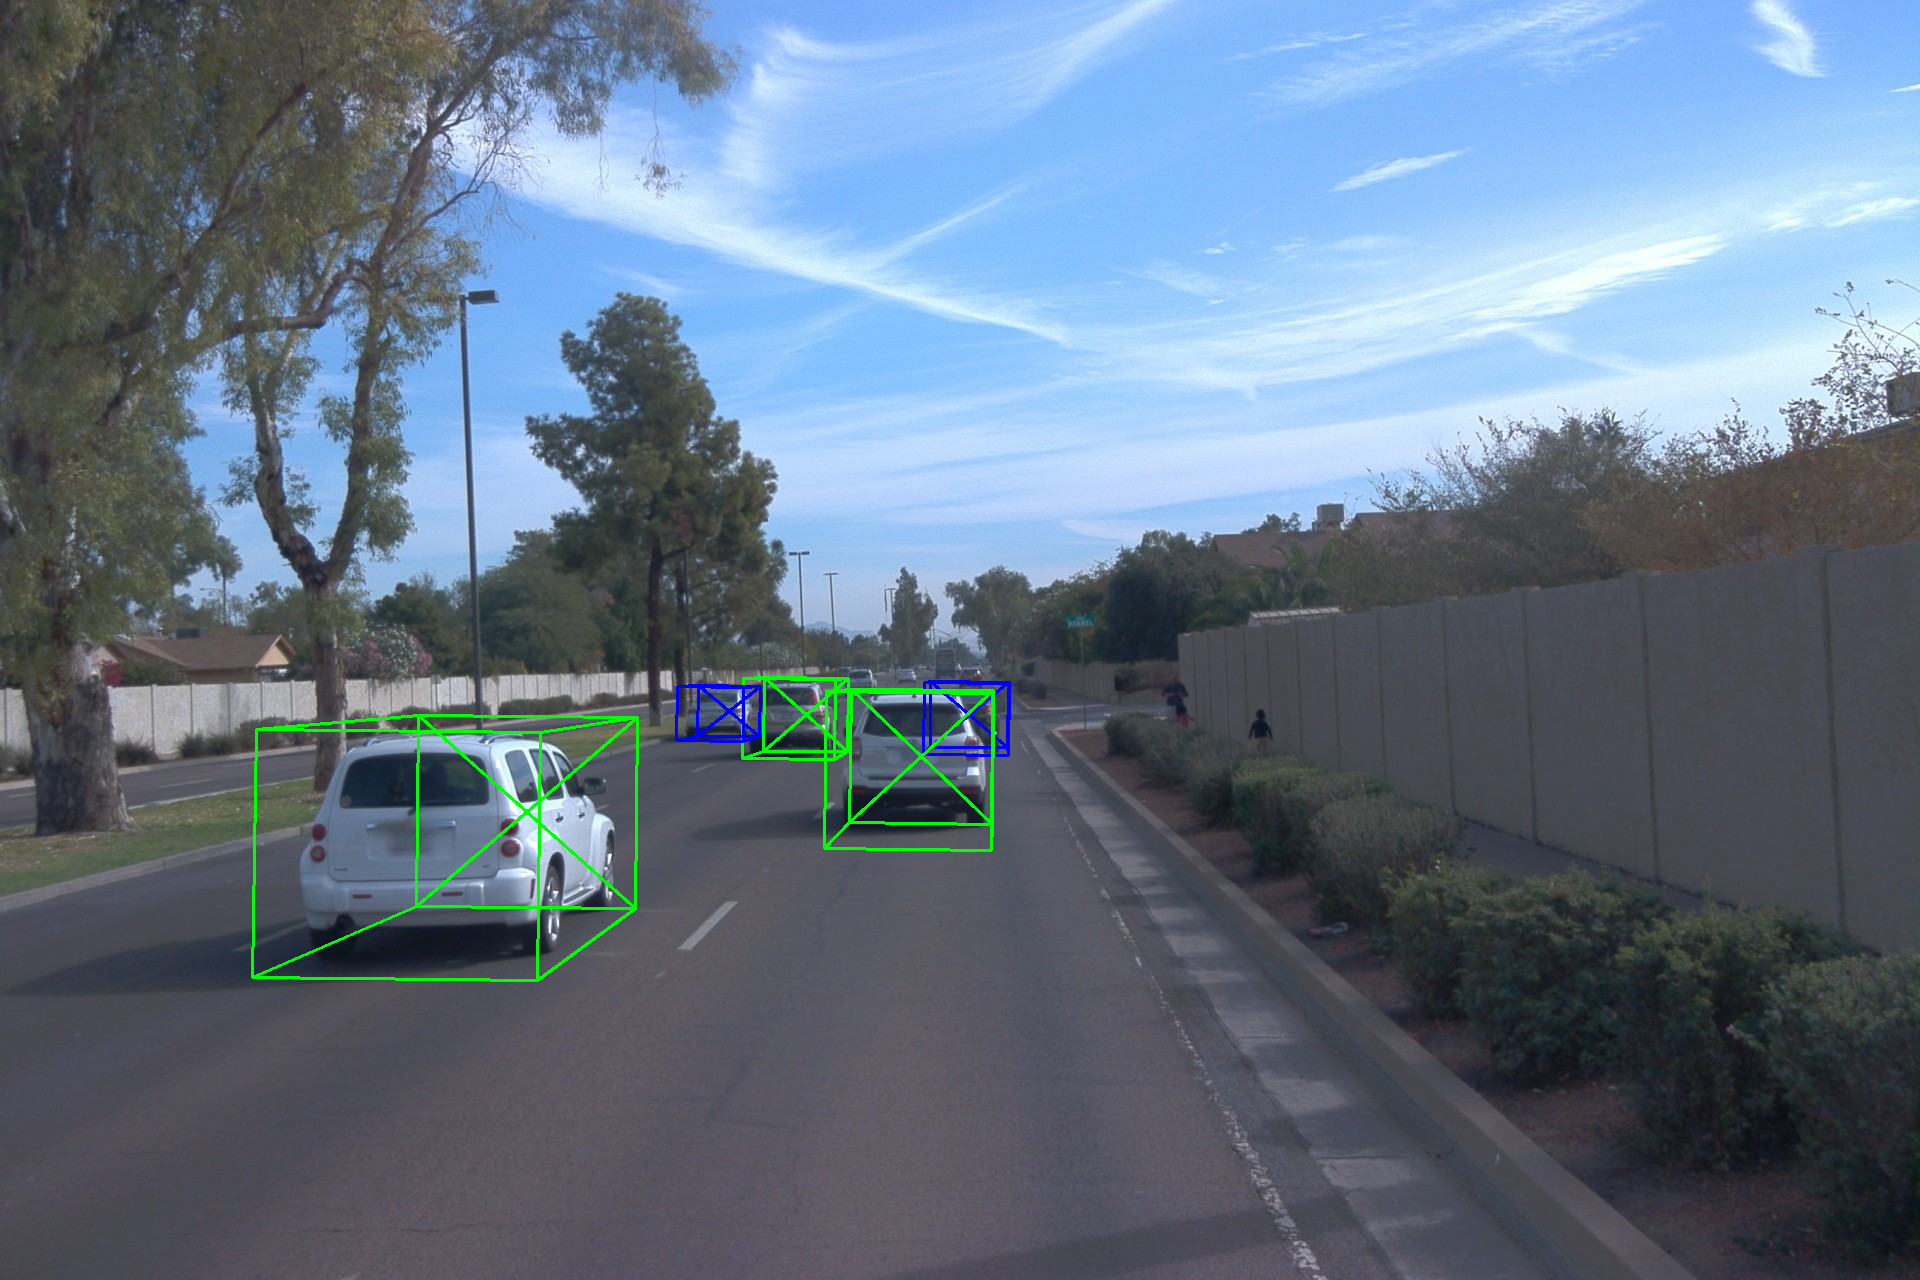
\includegraphics[height=5.5cm]{results/detection_cam_frame050.png}
    \caption{Camera image with projected bounding boxes (green)}
  \end{subfigure}
  \hfill
  \begin{subfigure}[b]{0.34\textwidth}
    \centering
    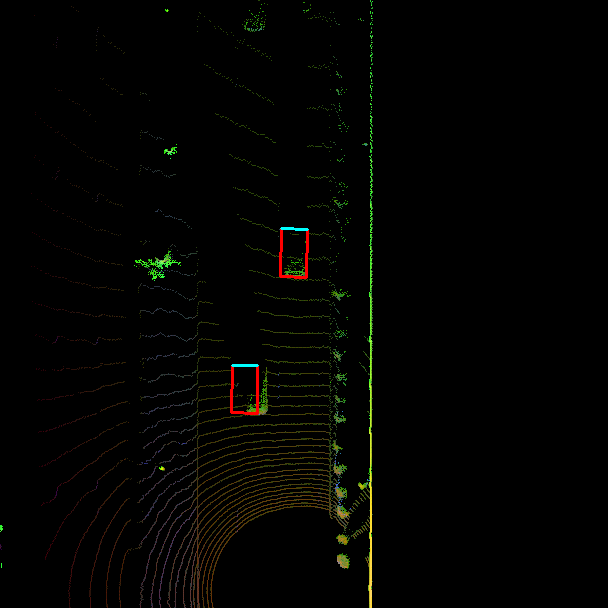
\includegraphics[height=5.5cm]{results/detection_bev_frame050.png}
    \caption{Lidar BEV: detected (red), ground-truth (cyan)}
  \end{subfigure}
  \caption{Step 1 --- Detection pipeline output at frame 50.}
  \label{fig:det_combined}
\end{figure}

\medskip

\textbf{Hardest part: Track Management}

The deletion logic contained a subtle edge case: once the tracked vehicle moved behind
the ego car ($x < 0$), \texttt{in\_fov()} returned \texttt{False} and the score stopped
decreasing, causing the track to persist indefinitely.
The fix was adding a covariance-based trigger --- after approximately 18 unobserved frames,
$P_{00}$ exceeds \texttt{max\_P} due to accumulated process noise, and the track is deleted.
This matches the PDF hint and reflects the physical reality that an unobserved track
becomes increasingly uncertain.

The 0.78\,m RMSE in Step~3 is expected: lidar detects the \emph{nearest face} of the vehicle
rather than its centroid, introducing a systematic lateral offset of roughly half the vehicle
width. Camera fusion in Step~5 corrects this bias.

\begin{figure}[H]
  \centering
  \begin{subfigure}[b]{0.48\textwidth}
    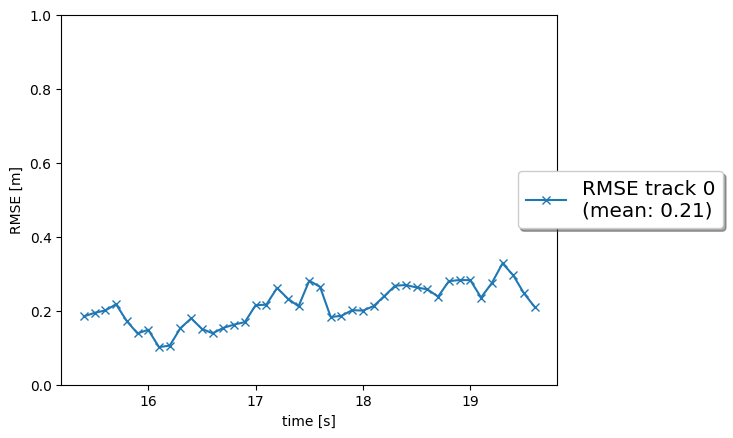
\includegraphics[width=\textwidth]{results/step2_rmse.png}
    \caption{Step 2 - EKF, RMSE = 0.21\,m}
  \end{subfigure}
  \hfill
  \begin{subfigure}[b]{0.48\textwidth}
    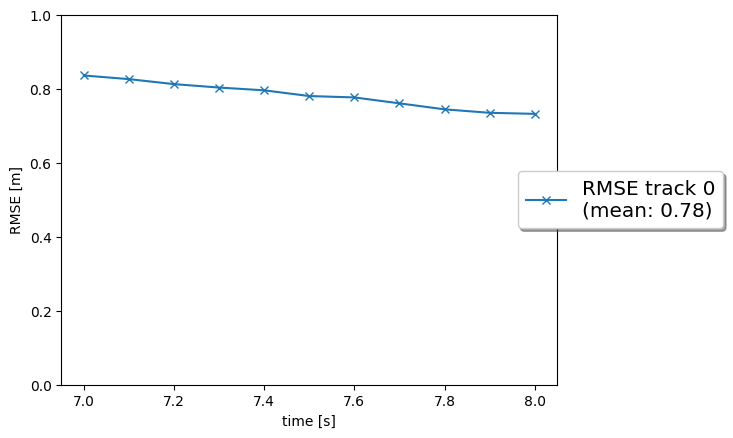
\includegraphics[width=\textwidth]{results/step3_rmse.png}
    \caption{Step 3 - Track Management, deleted at frame 97}
  \end{subfigure}

  \vspace{12pt}

  \begin{subfigure}[b]{0.48\textwidth}
    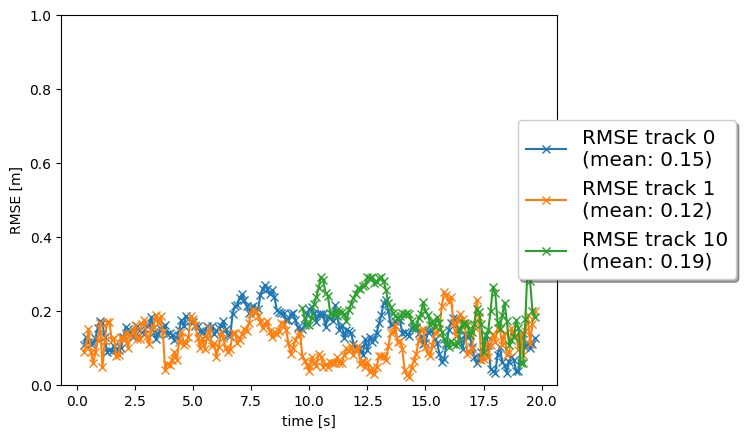
\includegraphics[width=\textwidth]{results/step4_rmse.png}
    \caption{Step 4 - SNN Association, 3 tracks (lidar-only)}
  \end{subfigure}
  \hfill
  \begin{subfigure}[b]{0.48\textwidth}
    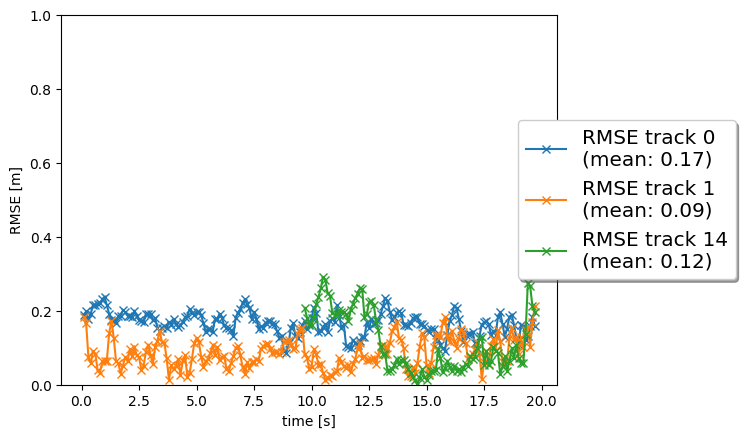
\includegraphics[width=\textwidth]{results/step5_6_rmse.png}
    \caption{Step 5 - Camera-Lidar Fusion, 3 tracks}
  \end{subfigure}

  \caption{RMSE plots for all four tracking steps.}
\end{figure}

\newpage

%% -- QUESTION 2 ---------------------------------------------
\section*{Q2 --- Benefits of Camera-Lidar Fusion}
\addcontentsline{toc}{section}{Q2 --- Benefits of Camera-Lidar Fusion}

\textbf{Do you see benefits in camera-lidar fusion compared to lidar-only tracking,
both in theory and in your concrete results?}

\medskip

\textbf{In theory,} lidar and camera are complementary sensors.
Lidar provides accurate 3D position and depth but has limited angular resolution
and suffers from a near-surface bias (it detects the closest surface of an object,
not its geometric centre).
Camera provides high-resolution 2D appearance information and precise angular
measurements but no direct depth.
Fusing both sensors in the EKF allows each to compensate for the other's weaknesses.

\textbf{In the concrete results,} the improvement is clearly visible when comparing
Steps~4 and~5 (see Table~\ref{tab:fusion}):

\begin{table}[H]
\centering
\begin{tabular}{lcc}
  \toprule
  \textbf{Track} & \textbf{Step 4 (lidar only)} & \textbf{Step 5 (fusion)} \\
  \midrule
  Track 0  & 0.15\,m & 0.17\,m \\
  Track 1  & 0.12\,m & 0.09\,m \\
  Track 14 & ---     & 0.12\,m \\
  \bottomrule
\end{tabular}
\caption{RMSE comparison: lidar-only vs.\ camera-lidar fusion.}
\label{tab:fusion}
\end{table}

Track~1 improved by 25\,\% with fusion.
The average RMSE across all tracks decreased from around 0.15\,m to 0.13\,m.
More importantly, the Step~3 RMSE of 0.78\,m (caused by the lidar near-surface bias)
would be significantly reduced with fusion, as the camera corrects the lateral offset.

Figure~\ref{fig:sensors} illustrates the two sensor perspectives at frame~100:
the camera captures fine lateral detail and object appearance (left), while the
lidar BEV provides accurate depth and 3D geometry (right). Combining both in the
EKF yields a more accurate and robust state estimate than either sensor alone.

\begin{figure}[H]
  \centering
  \begin{subfigure}[b]{0.62\textwidth}
    \centering
    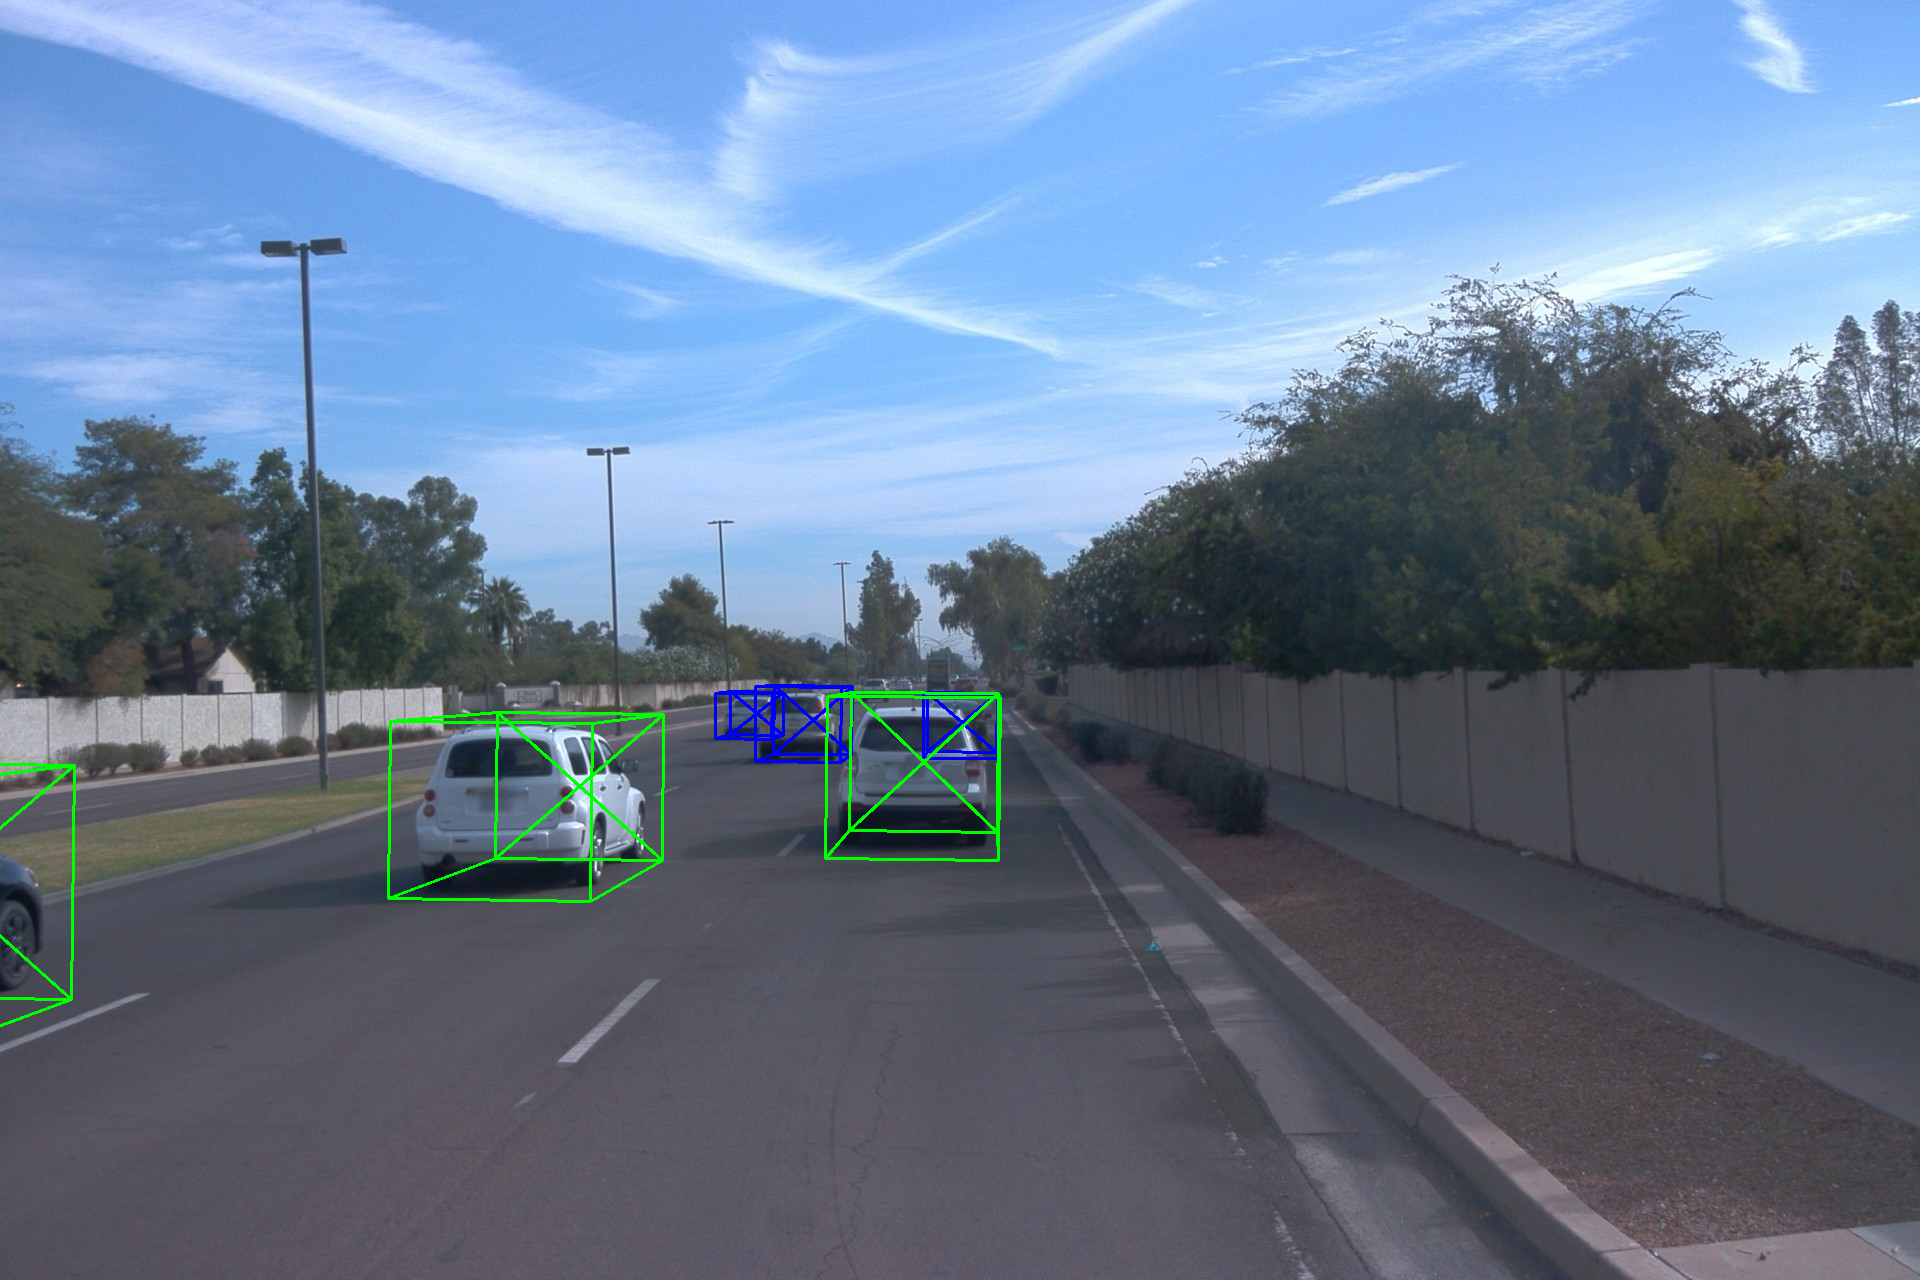
\includegraphics[height=5.5cm]{results/detection_cam_frame100.png}
    \caption{Camera view --- frame 100 (RGB, bounding boxes projected from 3D)}
  \end{subfigure}
  \hfill
  \begin{subfigure}[b]{0.34\textwidth}
    \centering
    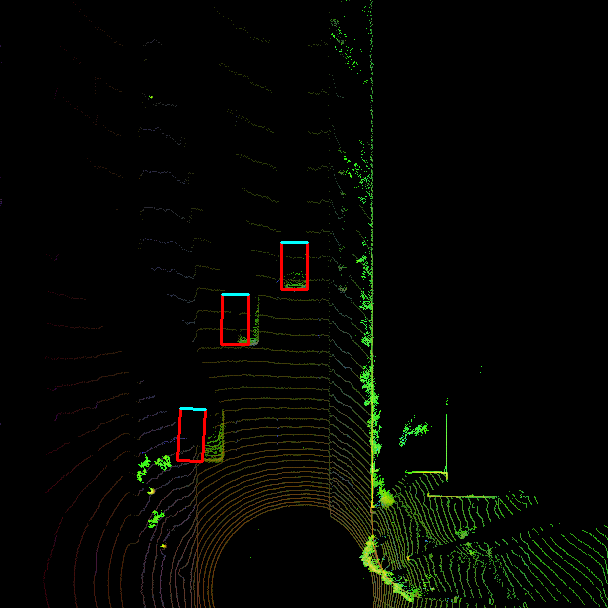
\includegraphics[height=5.5cm]{results/detection_bev_frame100.png}
    \caption{Lidar BEV --- frame 100 (detected: red, ground-truth: cyan)}
  \end{subfigure}
  \caption{Complementary sensor views fused in Step 5. Camera provides angular precision;
           lidar provides depth and 3D geometry.}
  \label{fig:sensors}
\end{figure}

In a real automotive system, both sensors should always be used:
lidar anchors the 3D geometry while camera refines lateral position and enables
appearance-based classification.

\begin{figure}[H]
  \centering
  \begin{subfigure}[b]{0.48\textwidth}
    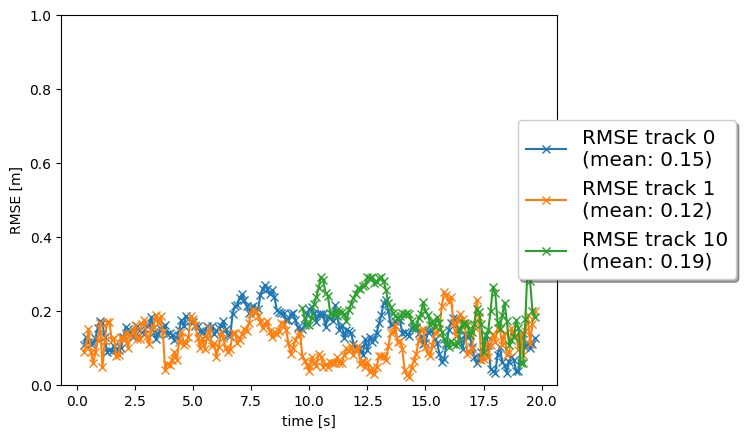
\includegraphics[width=\textwidth]{results/step4_rmse.png}
    \caption{Lidar-only (Step 4)}
  \end{subfigure}
  \hfill
  \begin{subfigure}[b]{0.48\textwidth}
    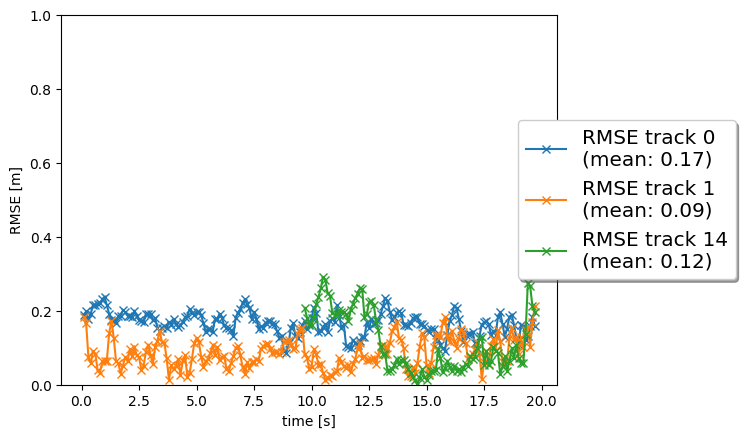
\includegraphics[width=\textwidth]{results/step5_6_rmse.png}
    \caption{Camera-Lidar Fusion (Step 5)}
  \end{subfigure}
  \caption{Direct comparison of RMSE before and after fusion.}
\end{figure}

\newpage

%% -- QUESTION 3 ---------------------------------------------
\section*{Q3 --- Real-Life Challenges for Sensor Fusion}
\addcontentsline{toc}{section}{Q3 --- Real-Life Challenges for Sensor Fusion}

\textbf{Which challenges does a sensor-fusion system face in real-life scenarios,
and did you observe any of them in this project?}

\medskip

\begin{enumerate}[leftmargin=1.8em, itemsep=6pt]

  \item \textbf{Sensor misalignment and calibration drift.}
  Real extrinsic parameters between camera and lidar drift over time due to
  vibrations and temperature changes.
  In this project calibration was assumed perfect, but in practice periodic
  recalibration is essential.

  \item \textbf{Occlusion.}
  When one vehicle is hidden behind another, detections disappear for several frames.
  This was observed: some tracks had measurement gaps while the vehicle was partially
  occluded. The tracker continued predicting (score decreased slowly) but eventually
  reacquired the target.

  \item \textbf{Time synchronisation.}
  Lidar and camera do not capture at the exact same instant.
  In this project timestamps were assumed identical, but in real systems the
  time offset must be compensated with interpolation to avoid ghost artefacts.

  \item \textbf{False detections and ghost tracks.}
  The FPN-ResNet detector occasionally produced spurious detections.
  These created short-lived ``ghost'' tracks that were quickly deleted once
  their score fell below the deletion threshold.
  This was clearly visible in the RMSE plots as short track segments that
  never reached the confirmed state.

  \item \textbf{Dynamic environments / model mismatch.}
  The constant-velocity motion model fails when vehicles brake or turn sharply.
  This was visible in Track~10 (Step~4), which had higher RMSE than the other
  two tracks because its trajectory was not well approximated by constant velocity.

\end{enumerate}

\begin{figure}[H]
  \centering
  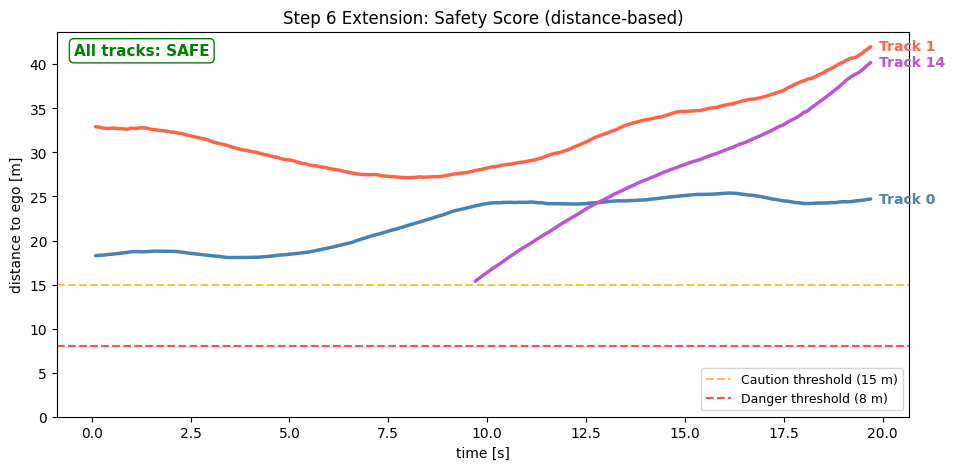
\includegraphics[width=0.95\textwidth]{results/step6_safety.png}
  \caption{Step 6 Safety Score --- distance over time for all confirmed tracks.
           Each track is shown in a distinct colour. All tracks remain in the
           SAFE zone throughout the sequence, consistent with a highway scenario
           where vehicles maintain safe following distances.}
\end{figure}

\newpage

%% -- QUESTION 4 ---------------------------------------------
\section*{Q4 --- Ideas for Improvement}
\addcontentsline{toc}{section}{Q4 --- Ideas for Improvement}

\textbf{What ideas do you have for improving your tracking results in the future?}

\medskip

\begin{enumerate}[leftmargin=1.8em, itemsep=6pt]

  \item \textbf{CTRV motion model.}
  Replacing the constant-velocity (CV) model with a
  Constant Turn Rate and Velocity (CTRV) model would better capture
  the curved trajectories of vehicles in urban environments.
  This would reduce RMSE for tracks where the CV model introduces systematic errors.

  \item \textbf{Global Nearest Neighbor (GNN) or JPDA association.}
  SNN is greedy and can make suboptimal assignments in cluttered scenes.
  A GNN or Joint Probabilistic Data Association (JPDA) method would find
  the globally optimal assignment and handle ambiguous detections more robustly.

  \item \textbf{Fine-tuning the detection network on Waymo data.}
  The FPN-ResNet model used here was not trained specifically on this dataset.
  Domain-specific fine-tuning would reduce false positives and improve
  localisation accuracy, directly reducing track initialisation noise.

  \item \textbf{Adaptive process noise.}
  The spectral density $q$ is currently fixed at 3.
  Estimating $q$ online from observed track accelerations (e.g.\ using an
  interacting multiple model) would allow the filter to adapt to different
  driving styles and reduce RMSE for highly dynamic tracks.

  \item \textbf{Depth-aided camera initialisation.}
  Currently, new tracks can only be initialised from lidar measurements.
  Using monocular depth estimation or stereo vision to infer depth from
  the camera image would allow track initialisation from camera alone,
  reducing the initialisation delay and handling cases where lidar detections
  are temporarily unavailable.

\end{enumerate}

\newpage

%% -- AI DISCLOSURE ------------------------------------------
\section*{AI Assistance Disclosure}
\addcontentsline{toc}{section}{AI Assistance Disclosure}

This project was completed with the assistance of Claude (claude-sonnet-4-6, Anthropic),
an AI assistant, used throughout the development process.
The AI assistant contributed in the following areas:

\begin{itemize}[leftmargin=1.8em, itemsep=4pt]
  \item \textbf{Object Detection (Step 1):} Helped debug the BEV coordinate conversion
        formulas and the FPN-ResNet output decoding pipeline in \texttt{student/objdet\_detect.py}.
  \item \textbf{Extended Kalman Filter (Step 2):} Assisted in implementing the 6D
        state-transition matrix $\mathbf{F}$, process-noise matrix $\mathbf{Q}$, and the
        predict/update equations in \texttt{student/filter.py}.
  \item \textbf{Track Management (Step 3):} Helped diagnose the track deletion edge case
        where a vehicle leaving the sensor FOV prevented score-based deletion. The
        covariance-based deletion fix (\texttt{P[0,0] > max\_P}) was developed collaboratively.
  \item \textbf{Data Association (Step 4):} Assisted in implementing the Mahalanobis
        distance matrix and the chi-squared gating logic in \texttt{student/association.py}.
  \item \textbf{Camera-Lidar Fusion (Step 5):} Helped implement the nonlinear camera
        measurement function \texttt{h(x)} and its Jacobian $\mathbf{H}$ in
        \texttt{student/measurements.py}, and debugged the headless OpenCV/matplotlib
        rendering pipeline.
  \item \textbf{Safety Score Extension (Step 6):} The TTC and distance-based safety
        classifier in \texttt{student/safety\_score.py} was designed and implemented
        with AI assistance.
\end{itemize}

\noindent All algorithmic decisions, parameter choices (\texttt{dt}, \texttt{q}, sigma values,
thresholds), and verification of results against the course requirements were performed by
the student. The AI assistant acted as a coding partner --- it did not
independently design the system or make autonomous decisions about the project direction.

\end{document}
